%%%%%%%%%%%%%%%%%%%%%%%%%%%%%%%%%%%%%%%%%%%%%%%%%%%%%%%%%%%%%%%%%%%%%%%%%%%
% Beamer Presentation
% LaTeX Template
% Version 2.0 (March 8, 2022)
%
% This template originates from:
% https://www.LaTeXTemplates.com
%
% License:
% CC BY-NC-SA 4.0 (https://creativecommons.org/licenses/by-nc-sa/4.0/)
%
%%%%%%%%%%%%%%%%%%%%%%%%%%%%%%%%%%%%%%%%%%%%%%%%%%%%%%%%%%%%%%%%%%%%%%%%%%%
%%%%%%%%%%%%%%%%%%%%%%%%%%%%%%%%%%%%%%%%%%%%%%%%%%%%%%%%%%%%%%%%%%%%%%%%%%%
%
%%%%%%%%%%%%%%%%%%%%%%%%% MADE BY RICARDO CHIN %%%%%%%%%%%%%%%%%%%%%%%%%%%%
%
%%%%%%%%%%%%%%%%%%%%%%%%%%%%%%%%%%%%%%%%%%%%%%%%%%%%%%%%%%%%%%%%%%%%%%%%%%%
%%%%%%%%%%%%%%%%%%%%%%%%%%%%%%%%%%%%%%%%%%%%%%%%%%%%%%%%%%%% December 2023
%
% github.com/roaked 
% ricardochin.com
%                                                          git: MIT License
%----------------------------------------------------------------------------------------
%	PACKAGES AND OTHER DOCUMENT CONFIGURATIONS
%----------------------------------------------------------------------------------------

\documentclass[
	11pt, 
]{beamer}

\graphicspath{{Images/}{./}} 
\usepackage{graphicx}
\usepackage{booktabs} 
\usepackage{tikz}
\usetikzlibrary{shapes.arrows}
% Allows the use of \toprule, \midrule and \bottomrule for better rules in tables

\tikzset{
    myarrow/.style={
        draw,
        fill=orange,
        single arrow,
        minimum height=3.5ex,
        single arrow head extend=1ex
    }
}
\newcommand{\arrowup}{%
\tikz [baseline=-0.5ex]{\node [myarrow,rotate=90] {};}
}
\newcommand{\arrowdown}{%
\tikz [baseline=-1ex]{\node [myarrow,rotate=-90] {};}
}


%----------------------------------------------------------------------------------------
%	SELECT LAYOUT THEME
%----------------------------------------------------------------------------------------

\usetheme{Boadilla} %ok
%\usetheme{CambridgeUS} %red
%\usetheme{Goettingen} % ok
%\usetheme{Singapore} %good
%\usetheme{Szeged} %good

%----------------------------------------------------------------------------------------
%	SELECT COLOR THEME
%----------------------------------------------------------------------------------------


\usecolortheme{seahorse}


%----------------------------------------------------------------------------------------
%	SELECT FONT THEME & FONTS
%----------------------------------------------------------------------------------------

\usefonttheme{default}

%\usepackage{mathptmx} % Use the Times font for serif text
\usepackage{palatino} % Use the Palatino font for serif text
%\usepackage{helvet} % Use the Helvetica font for sans serif text
\usepackage[default]{opensans} % Use the Open Sans font for sans serif text
%\usepackage[default]{FiraSans} % Use the Fira Sans font for sans serif text
%\usepackage[default]{lato} % Use the Lato font for sans serif text

%----------------------------------------------------------------------------------------
%	SELECT INNER THEME
%----------------------------------------------------------------------------------------

%\useinnertheme{default}
\useinnertheme{circles}
%\useinnertheme{rectangles}
%\useinnertheme{rounded}
%\useinnertheme{inmargin}

%----------------------------------------------------------------------------------------
%	SELECT OUTER THEME
%----------------------------------------------------------------------------------------

%\useoutertheme{default}
%\useoutertheme{infolines}
%\useoutertheme{miniframes}
%\useoutertheme{smoothbars}
%\useoutertheme{sidebar}
%\useoutertheme{split}
%\useoutertheme{shadow}
%\useoutertheme{tree}
%\useoutertheme{smoothtree}

%----------------------------------------------------------------------------------
%	PRESENTATION INFORMATION
%----------------------------------------------------------------------------------

\title[Python: Intermediate Fundamentals]{Intermediate Workshop to Python Programming}
\subtitle{Building the Foundation for Coding Success}
\author[Ricardo Chin]{Ricardo Chin}

\begin{document}
\begin{frame}
    \titlepage
    \begin{figure}
        
\includegraphics[width=0.1\linewidth]{5848152fcef1014c0b5e4967}
    \end{figure}
    \frametitle{Workshop Details}
\end{frame}

%----------------------------------------------------------------------------------
%	TABLE OF CONTENTS SLIDE
%----------------------------------------------------------------------------------

\begin{frame}
	\frametitle{Presentation Overview}
	
	\tableofcontents
	%\tableofcontents[pausesections] % Output the table of contents (break sections up across separate slides)
\end{frame}


%%%%%%%%%%%%%%%%%%%%%%%%%%%%%%%%%%%%%%%%%%%%%%%%%%%%%%%%%%%%%%%%%%%%%%%%%%%%%%%

\section{Numeric Data Types} %change
\begin{frame}[fragile]{Data Types: Deeper Dive} %change

\begin{center}
--- Previously in \textsc{Python Programming} ---

\vspace{.25cm}
\arrowdown
\end{center}

\begin{itemize}
    \item \texttt{int}: Whole numbers without decimal points
    \item \texttt{float}: Numbers with decimal points
    \item \texttt{bool}: Represents the truth values \texttt{True} or \texttt{False}
    \item \texttt{NoneType} (\texttt{None}): Represents absence of a value (or null)
    \item \texttt{string}: Ordered sequence of characters 
\end{itemize}

\vspace{.2cm}

\textbf{Collections}
\begin{itemize}
    \item \texttt{list}: Ordered and mutable sequence of elements
    \item \texttt{tuple}: Ordered and immutable sequence of elements
    \item \texttt{dict}: Unordered collection of key-value pairs
\end{itemize}

\end{frame}

%%%%%%%%%%%%%%%%%%%%%%%%%%%%%%%%%%%%%%%%%%%%%%%%%%%%%%%%%%%%%%%%%%%%%%%%%%%%%%%

\begin{frame}[fragile]{NoneType} %change

\textbf{NoneType}
\begin{itemize}
    \item \texttt{None} is a Singleton --- there is only ever a single instance of it inside a running Python program
    \item Multiple variables may refer to that same instance
\end{itemize}

\vspace{.2cm}

\textbf{Comparisons using Keyword \texttt{"is"}}

\vspace{.2cm}

Keyword \texttt{is} checks whether two names refer to the same object

\vspace{.4cm}

\begin{minipage}[t]{0.30\textwidth}
\begin{verbatim}
    a = [1, 2]
    b = a
    x = [1, 2]
    
    a == b # True
    a is b # True
    a == x # True
    a is x # False
\end{verbatim}
\end{minipage}
\hfill
\begin{minipage}[t]{0.50\textwidth}
As \texttt{None} is a singleton, we can check for it via \texttt{is None}

\begin{verbatim}
if a is None:
    print("a is None")
\end{verbatim}

\end{minipage}
\end{frame}

%%%%%%%%%%%%%%%%%%%%%%%%%%%%%%%%%%%%%%%%%%%%%%%%%%%%%%%%%%%%%%%%%%%%%%%%%%%%%%%

\begin{frame}[fragile]{BoolType} %change

\textbf{BoolType}
\vspace{.2cm}
\begin{itemize}
    \item The \texttt{bool} type is a built-in data type representing truth values
    \item It has two possible values: \texttt{True} and \texttt{False}
\end{itemize}

\begin{minipage}[t]{0.30\textwidth}
\begin{verbatim}
a = True
if a:
    print('hello')
\end{verbatim}
\end{minipage}
\hfill
\begin{minipage}[t]{0.62\textwidth}
    \begin{verbatim}
x, y = 10, 20
is_greater = x > y   # False
if is_greater:
    print("x greater than y")
else:
    print("x not greater than y")
    \end{verbatim}
\end{minipage}

Booleans are a subset of integers (subclass of int) where \texttt{True} behaves as 1 and \texttt{False} as 0 in numerical contexts

\centering
\vspace{.4cm}
\texttt{False + True # 1}

\end{frame}

%%%%%%%%%%%%%%%%%%%%%%%%%%%%%%%%%%%%%%%%%%%%%%%%%%%%%%%%%%%%%%%%%%%%%%%%%%%%%%%

\begin{frame}[fragile]{Numbers} %change

\begin{block}{\textbf{Operations with Numbers}}
    \begin{itemize}
        \item Integer Division: 10 // 3 = 3
        \item Remainder: 10 \% 3 = 1
        \item Exponentiation: 2 ** 3 = 8
    \end{itemize}
    
\end{block}
\vspace{.22cm}
\pause
\begin{center}
    \arrowdown
\end{center}
\vspace{.22cm}

\begin{block}{\textbf{Underscores in Numeric Literals for Enhanced Readibility}}
    \begin{itemize}
        \item Revenue: 1000000000
        \item Revenue: 1\_000\_000\_000
    \end{itemize}
    
\end{block}
    

\end{frame}

%%%%%%%%%%%%%%%%%%%%%%%%%%%%%%%%%%%%%%%%%%%%%%%%%%%%%%%%%%%%%%%%%%%%%%%%%%%%%%%

\begin{frame}[fragile]{Integer Type Representations} %change

\begin{block}{\textbf{Integers}}
\begin{enumerate}
    \item Python supports integers of arbitrary size, allowing representation of very large numbers 

    \item It also supports different numeral systems
    \vspace{.1cm}
    \begin{itemize}
        \item Decimal --- \texttt{a = 42}
        \item Binary ---  \texttt{b = 0b101010}
        \item Octal ---  \texttt{c = 0o52}
        \item Hexadecimal ---  \texttt{d = 0x2a}
        \item Conversion from a string in binary to an integer --- \texttt{e = int('101010', 2)}
    \end{itemize}

\end{enumerate}
\end{block}


\begin{exampleblock}{\textbf{Tip ---} Maximum Size of Integers on the Current System}
\vspace{.05cm}
    \begin{verbatim}
    import sys
    print(sys.maxsize)  # Maximum size
    \end{verbatim}
\end{exampleblock}

\end{frame}


%%%%%%%%%%%%%%%%%%%%%%%%%%%%%%%%%%%%%%%%%%%%%%%%%%%%%%%%%%%%%%%%%%%%%%%%%%%%%%%

\begin{frame}[fragile]{Float Type Representations} %change

\begin{block}{\textbf{Integers}}
\begin{enumerate}
    \item Floating-point numbers in Python use 64 bits
        \begin{itemize}
            \item \textbf{Numbering} --- \hspace{.1cm} \texttt{a = .12} \hspace{.1cm} or \hspace{.3cm} \texttt{b = 2.55}
            \item \textbf{Scientific Notation} --- \hspace{.1cm} \texttt{c = 6e23}
            \item \textbf{Special Values} --- \texttt{d = float('nan')}  or  \hspace{.1cm} \texttt{e = float('inf')}
        \end{itemize}


\end{enumerate}
\end{block}

\begin{figure}
    \centering
    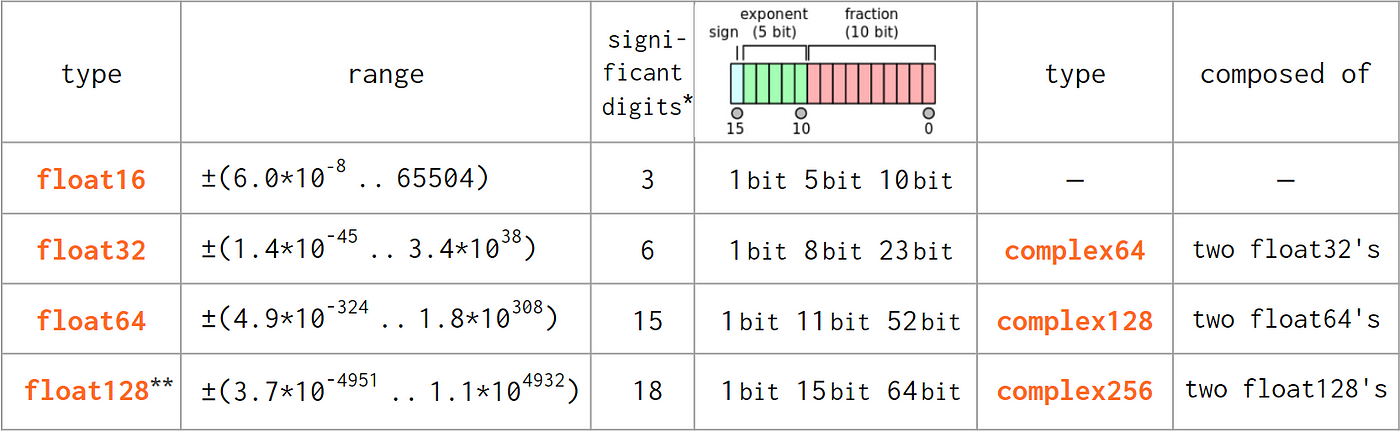
\includegraphics[width = 12cm]{Images/bits.png}
    \caption{Based on IEEE 754 --- Standardized Floating-point Arithmetic}
\end{figure}

\end{frame}

%%%%%%%%%%%%%%%%%%%%%%%%%%%%%%%%%%%%%%%%%%%%%%%%%%%%%%%%%%%%%%%%%%%%%%%%%%%%%%%

\begin{frame}[fragile]{Float Type Representations} %change

\begin{alertblock}{\textbf{Warning!}}
    Floating-point numbers, while versatile, can't perfectly represent all real numbers. This limitation leads to rounding errors, causing some numbers to be approximations rather than precise representations
\end{alertblock}

\pause
\begin{center}
    \arrowdown
\end{center}


In the decimal system:
\begin{enumerate}
    \item Fractions like 1/3 and 1/7 can't be represented exactly
    \item Constant like $\pi$ isn't fully representable without approximation
\end{enumerate}

In binary floats:
\begin{enumerate}
    \item Decimals like 1/2 and 1/10 can't be precisely represented
    \item Fractions like 1/3 and even π suffer from approximation
\end{enumerate}

\end{frame}

%%%%%%%%%%%%%%%%%%%%%%%%%%%%%%%%%%%%%%%%%%%%%%%%%%%%%%%%%%%%%%%%%%%%%%%%%%%%%%%

\begin{frame}[fragile]{Float Rounding Errors} %change

\begin{alertblock}{\textbf{Warning!}}
    As a consequence to not being able to perfectly represent all real numbers, float numbers will lead to rounding error mismatches
\end{alertblock}

\textbf{Example 1 --- Precision Limitations}
\begin{enumerate}
    \item Computing $\pi$ + $\pi$ might yield 6.2 when using decimal numbers with a precision of 2, whereas a more precise result would be 6.3
\end{enumerate}

\textbf{Example 1 --- Arithmetic Precision}
\begin{enumerate}
    \item Simple addition like 0.1 + 0.2 might oddly evaluate to $\approx$ 0.30000000000000004 due to limitations in 64-bit floats
\end{enumerate}
\vspace{.1cm}

\begin{verbatim}
0.1 + 0.2 == 0.3 # Returns False if float assigned

import math      # tolerance = 1e-09
math.isclose(0.1 + 0.2, 0.3) # Returns True
\end{verbatim}

\end{frame}


%%%%%%%%%%%%%%%%%%%%%%%%%%%%%%%%%%%%%%%%%%%%%%%%%%%%%%%%%%%%%%%%%%%%%%%%%%%%%%%

\begin{frame}[fragile]{Complex Type and Augmented Assignment} %change

A complex number is a numerical type used to represent numbers that have both a real part and an imaginary part: \texttt{a = 1 + 2j}

\vspace{.1cm}

\textbf{Let us increment the real part \texttt{(1)} of the variable $a$}

\[
a = a + 1 \hspace{.3cm} \texttt{or} \hspace{.3cm} a+= 1
\]

\begin{exampleblock}{\textbf{Augmented Assignment}}
This operation means "add 1 to the current value of $a$ and assign the result back to $a$ 
\end{exampleblock}

\vspace{.12cm}

Calculation:
\[
a = 1 + 2j + 1
\]

Result:
\[
a = 2 + 2j
\]

Other operations include: \hspace{.1cm} \texttt{-=, *=, ...}

\end{frame}

%%%%%%%%%%%%%%%%%%%%%%%%%%%%%%%%%%%%%%%%%%%%%%%%%%%%%%%%%%%%%%%%%%%%%%%%%%%%%%%

\section{Character Encodings}
\begin{frame}{Character Encodings}

Character encodings are used to represent characters in a form that computers can understand and manipulate --- mapping characters to bit sequences

\begin{block}{\textbf{Types of Character Encodings}}
     \begin{enumerate}
         \item ASCII (American Standard Code for Information Interchange)
         \begin{itemize}
             \item Encodes the first 128 Unicode characters using 7 bits, covering basic English characters, digits, and symbols
             \item Represents characters like 'A', '!', '\$', space, and line breaks
         \end{itemize}
         \item Latin1 (ISO 8859-1)
         \begin{itemize}
             \item Extends ASCII to encode the first 256 Unicode characters using 8 bits
             \item Adds additional characters like '$\ddot{a}$ ', '$á$ ', '$\beta$', '$\S$', etc
        
         \end{itemize}
         \item UTF-8, UTF-16, UTF-32
         \begin{itemize}
             \item Encode the entire Unicode character set
             \item UTF-8, a popular encoding, uses variable-width encoding
         \end{itemize}
     \end{enumerate}
\end{block}
    
\end{frame}

%%%%%%%%%%%%%%%%%%%%%%%%%%%%%%%%%%%%%%%%%%%%%%%%%%%%%%%%%%%%%%%%%%%%%%%%%%%%%%%

\begin{frame}{Character Encodings}

Examples in ASCII / Latin1 / UTF-8:

\begin{center}
\vspace{.1cm}
\begin{tabular}{|c|c|}
\hline
Character & Byte Representation \\
\hline
! & 00100001 \\
A & 01000001 \\
Line Feed | Line Break | "\textbackslash{}n" & 00001010 \\
\hline
\end{tabular}
\end{center}

Examples in Latin1:

\begin{center}
\vspace{.1cm}
\renewcommand{\arraystretch}{1.3}
\begin{tabular}{|c|c|}
\hline
Character & Byte Representation \\
\hline
$\ddot{A}$ & 11000100 \\
\hline
\end{tabular}
\end{center}

Examples in UTF-8:

\begin{center}
\vspace{.1cm}
\renewcommand{\arraystretch}{1.3}
\begin{tabular}{|c|c|}
\hline
Character & Byte Representation \\
\hline
$\ddot{A}$ & 11000011 10100100 \\
$\ddot\smile$ & 11110000 10011111 10011001 10000010 \\
\hline
\end{tabular}
\end{center}
    
\end{frame}

%%%%%%%%%%%%%%%%%%%%%%%%%%%%%%%%%%%%%%%%%%%%%%%%%%%%%%%%%%%%%%%%%%%%%%%%%%%%%%%

\begin{frame}{Strings}

Strings represent sequences of Unicode characters, allowing the manipulation and representation of text data

\begin{center}
    \arrowdown
\end{center}

\begin{enumerate}
    \item \textbf{String Literals} --- Representations of strings in Python
    \begin{itemize}
        \item Single quotes: \texttt{a = 'test'}
        \item Double quotes: \texttt{b = "test"}
    \end{itemize}
    \vspace{.3cm}

    \item \textbf{Multi-line String Literals} --- Multi-line representation 
    \texttt{\\
    a = """this\\
    is a multi-line\\
    string literal
    """}
    \vspace{.3cm}
    
    \item \textbf{Escape Sequences} --- \texttt{a = "He said:\textbackslash{}n\textbackslash{}"Hi!\textbackslash{}""} \\
    \textbackslash{}n for line feed or line break!
\end{enumerate}
    
\end{frame}

%%%%%%%%%%%%%%%%%%%%%%%%%%%%%%%%%%%%%%%%%%%%%%%%%%%%%%%%%%%%%%%%%%%%%%%%%%%%%%%

\begin{frame}[fragile]{Strings}

If there is no need to use any escape sequences in a string

\begin{verbatim}
    path = r"C:\documents\course\news.txt"
\end{verbatim}

Handy when writing directory paths and regular expressions

\begin{exampleblock}{Useful String Methods}
    \begin{itemize}
        \item \texttt{.lower()} and \texttt{.upper()}
        \item \texttt{.startswith(...)} and \texttt{.endswith(".xlsx")}
        \item \texttt{.center(10)} --- centered in 10 chars
        \item \texttt{.ljust(10)} --- left justified or \texttt{.rjust(10)} --- right justified
        \item \texttt{.strip()} --- removes leading and trailing spaces
        \item \texttt{.split(' ')} --- splits a string into a list of substrings
        \item \texttt{' '.join(list)} --- join a list of strings into a single string 
    \end{itemize}
\end{exampleblock}

\end{frame}

%%%%%%%%%%%%%%%%%%%%%%%%%%%%%%%%%%%%%%%%%%%%%%%%%%%%%%%%%%%%%%%%%%%%%%%%%%%%%%%

\begin{frame}[fragile]{String Exercises}

\begin{alertblock}{\textbf{Exercises}}
\begin{enumerate}
    \item Later
\end{enumerate}    
\end{alertblock}

\end{frame}


%%%%%%%%%%%%%%%%%%%%%%%%%%%%%%%%%%%%%%%%%%%%%%%%%%%%%%%%%%%%%%%%%%%%%%%%%%%%%%%

\begin{frame}[fragile]{String Formatting}

String formatting allows for the inclusion of values within strings

\begin{verbatim}
name = "Ricardo"     
# Concatenation
greeting = "Hello, " + name + "!"

# f-string (formatted string literals)
greeting = f"Hello, {name}!"
\end{verbatim}

There are other formatting ways which are currently a bit obsolete

\begin{verbatim}
city, temperature = 'Graz', 5.7    
'weather in %s: %f°C' % (city, temperature)
'weather in {0}: {1}°C'.format(city, temperature)
'weather in {}: {}°C'.format(city, temperature)
'weather in {c}: {t}°C'.format(c=city, t=temperature)
f'weather in {city}: {temperature}°C' # fstring pref
\end{verbatim}

\end{frame}

%%%%%%%%%%%%%%%%%%%%%%%%%%%%%%%%%%%%%%%%%%%%%%%%%%%%%%%%%%%%%%%%%%%%%%%%%%%%%%%

\begin{frame}[fragile]{Format Specifications}

If we want to specify the format value itself --- ie, \texttt{.4g} or \texttt{.4f}

\begin{verbatim}
# Four decimal places after the decimal point
print(f"Pi is {math.pi:.4f}") # Output: Pi is 3.1416

# Four significant digits
print(f"Pi is {math.pi:.4g}") # Output: Pi is 3.142
\end{verbatim}

If we want to specify the sentence alignment

\begin{verbatim}
first_name, last_name = "Ricardo", "Chin"

# Right-aligned (total width 8 characters)
print(f"{first_name:>8}")  # Output: " Ricardo"
print(f"{last_name:>8}")   # Output: "    Chin"
\end{verbatim}

\begin{itemize}
    \item \href{https://mkaz.blog/working-with-python/string-formatting/}{String Formatting Reference --- Hyperlink}
\end{itemize}

\end{frame}

%%%%%%%%%%%%%%%%%%%%%%%%%%%%%%%%%%%%%%%%%%%%%%%%%%%%%%%%%%%%%%%%%%%%%%%%%%%%%%%

\section{Interesting References}
\begin{frame}[fragile]{Interesting References}
\begin{exampleblock}{\textbf{Books}}
    
\begin{itemize}


\item \href{https://automatetheboringstuff.com/}{Automate the Boring Stuff with Python by Al Sweigart}

\item \href{http://greenteapress.com/thinkpython2/thinkpython2.pdf}{Think Python, 2nd Edition by Allen B. Downey}

\item \href{https://www.py4e.com/book.php}{Python for Everybody by Dr. Charles Severance}

\end{itemize}
\end{exampleblock}

\begin{exampleblock}{\textbf{Online Courses and Tutorials}}

\begin{itemize}

\item \href{https://mkaz.blog/working-with-python/string-formatting/}{String Formatting}

\item \href{https://www.codecademy.com/learn/learn-python-3}{Codecademy - Beginner Course}

\item \href{https://learnxinyminutes.com/docs/python/}{Learn X in Y Minutes - Python}

\item \href{https://ehmatthes.github.io/pcc_2e/cheat_sheets/cheat_sheets/}{Python Cheat Sheets by Eric Matthes}
\end{itemize}
\end{exampleblock}
\end{frame}


%%%%%%%%%%%%%%%%%%%%%%%%%%%%%%%%%%%%%%%%%%%%%%%%%%%%%%%%%%%%%%%%%%%%%%%%%%%%%%%

\begin{frame}[fragile]{The End}

\centering

\Huge Thank you!

\end{frame}


%------------------------------------------------

% \subsection{Columns}

% \begin{frame}
% 	\frametitle{Multiple Columns}
% 	\framesubtitle{Subtitle} % Optional subtitle
	
% 	\begin{columns}[c] % The "c" option specifies centered vertical alignment while the "t" option is used for top vertical alignment
% 		\begin{column}{0.45\textwidth} % Left column width
% 			\textbf{Heading}
% 			\begin{enumerate}
% 				\item Statement
% 				\item Explanation
% 				\item Example
% 			\end{enumerate}
% 		\end{column}
% 		\begin{column}{0.5\textwidth} % Right column width
% 			Lorem ipsum dolor sit amet, consectetur adipiscing elit. Integer lectus nisl, ultricies in feugiat rutrum, porttitor sit amet augue. Aliquam ut tortor mauris. Sed volutpat ante purus, quis accumsan dolor.
% 		\end{column}
% 	\end{columns}
% \end{frame}

\end{document} 